\subsection{Performance}\label{subsec:IO_Subsystem_Performance}
I/O is a major factor in system performance.
\begin{itemize}[noitemsep]
\item It places heavy demands on the CPU to execute \nameref{def:Device_Driver} code and to schedule \nameref{def:Process}es fairly and efficiently as they block and unblock.
  \begin{itemize}[noitemsep]
  \item The resulting \nameref{def:Context_Switch}es stress the CPU and its hardware caches.
\end{itemize}
\item I/O exposes inefficiencies in the \nameref{def:Interrupt_Handler} mechanisms in the \nameref{def:Kernel}.
\item I/O loads down the memory bus during data copies between \nameref{def:Controller}s and \nameref{def:Physical_Memory} and again during copies between kernel buffers and application data space.
\end{itemize}

Coping gracefully with all these demands is one of the major concerns of the OS designer/architect.

Interrupt handling is a relatively expensive task.
Each interrupt causes the system to perform a state change, to execute the interrupt handler, and then to restore state.
Network traffic can also cause a high context-switch rate (see \Cref{fig:Intercomputer_Communications}).

\begin{figure}[h!tbp]
  \centering
  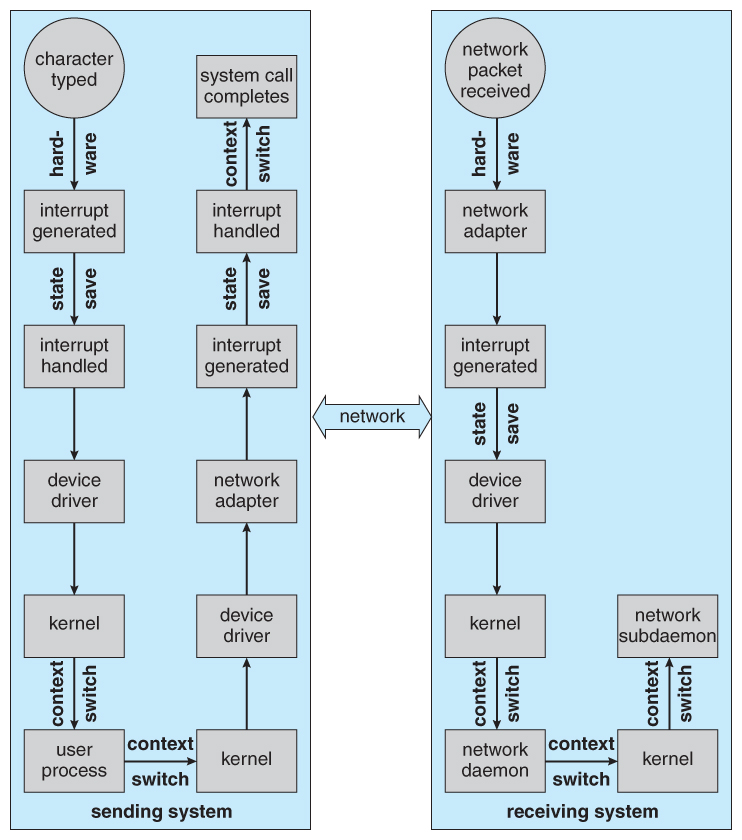
\includegraphics[scale=1.00]{./Drawings/EDAF35-Operating_Systems/Intercomputer_Communications.jpg}
  \caption{Intercomputer Communications}
  \label{fig:Intercomputer_Communications}
\end{figure}


%%% Local Variables:
%%% mode: latex
%%% TeX-master: "../../EDAF35-Operating_Systems-Reference_Sheet"
%%% End:
